%\documentclass[12pt,handout]{beamer}
\documentclass[xcolor=dvipsnames,presentation]{beamer}
\usepackage{../oop-slides-lab}
\setbeamertemplate{bibliography item}[text]

\newcommand{\lab}{Lab01}

\title[{\lab} -- Introduzione]{Introduzione al laboratorio}

\date[\today]{\today}

\begin{document}

\frame[label=coverpage]{\titlepage}

\begin{frame}<beamer>
	\frametitle{Outline}
	\tableofcontents[]
\end{frame}

\section{Organizzazione del Laboratorio}\label{sec:organizzazione-del-laboratorio}

\begin{frame}{Organizzazione del Laboratorio}
    \begin{itemize}
        \item Due turni settimanali
        \item Il contenuto della lezione e dell'esecitazione settimanale del laboratorio è il medesimo per entrambi i turni
        \item La gestione della partecipazione ai turni è demandata al prof. Viroli
        %\item Nello stesso giorno avrete sia OOP che OS
    \end{itemize}
    \begin{block}{Primo Turno (iniziale cognome nell'intervallo [A-G])}
        \begin{itemize}
            \item Lunedì, 9:00 - 13:00
            \item Lab. 2.2, Campus Cesena
        \end{itemize}
    \end{block}
    \begin{block}{Secondo Turno (iniziale cognome nell'intervallo [H-Z])}
        \begin{itemize}
            \item Martedì, 13:00 - 17:00
            \item Lab. 2.2, Campus Cesena
        \end{itemize}
    \end{block}
%    Potrà seguire IN PRESENZA chi è selezionato su ``Presente'' per seguire in presenza. Tutti gli altri dovranno seguire online, nel giorno assegnato.
\end{frame}

% \begin{frame}{Turni e app ``Presente''}
%     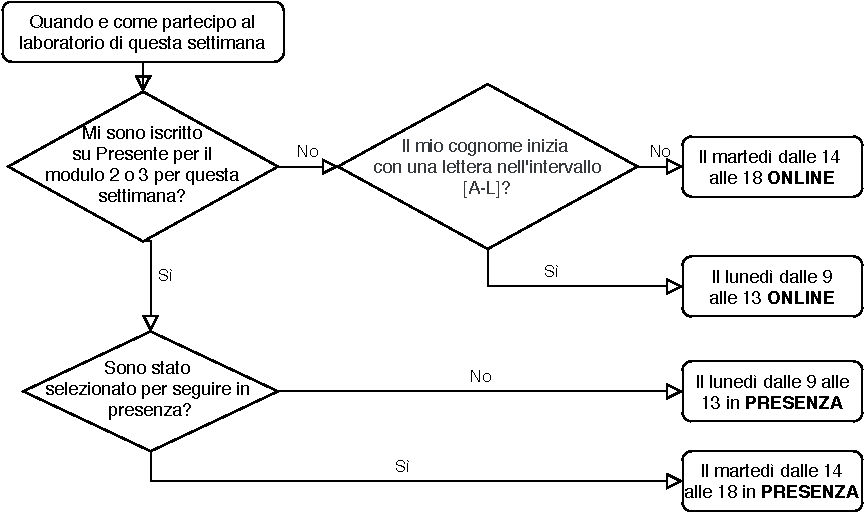
\includegraphics[width=\textwidth]{img/covid-presente}
% \end{frame}

\begin{frame}{Docenti del Laboratorio}
    \begin{block}{Prof. Danilo Pianini -- Responsabile Modulo 2}
        \begin{itemize}
            \item mail: \texttt{danilo.pianini@unibo.it}
            \item ricevimento: su appuntamento, da concordare via mail
        \end{itemize}
    \end{block}
    \begin{block}{Prof. Roberto Casadei -- Responsabile Modulo 3}
        \begin{itemize}
            \item mail: \texttt{roby.casadei@unibo.it}
            \item ricevimento: su appuntamento, da concordare via mail
        \end{itemize}
    \end{block}
    \begin{block}{Ing. Luca Deluigi -- Tutor Didattico}
        \begin{itemize}
            \item mail: \texttt{luca.deluigi5@unibo.it}
        \end{itemize}
    \end{block}
%    \begin{block}{Ing. Luca Tremamunno -- Tutor Didattico}
%        \begin{itemize}
%            \item mail: \texttt{luca.tremamunno@unibo.it}
%        \end{itemize}
%    \end{block}
\end{frame}

\section{Forum e supporto}

\begin{frame}{Il Laboratorio}

\begin{itemize}
    \item Consente di mettere in pratica quanto visto nelle lezioni in aula
    \begin{itemize}
    	\item lo studente affronta gli esercizi in prima persona (\textbf{approccio attivo}) 
        \item lo studente può (ed è invitato a) richiedere il supporto diretto dei pari, del tutor, e del docente \textbf{approccio cooperativo}
    \end{itemize}
    \item Integra ed espande i contenuti affrontati in aula
    \item Introduce \textbf{nuovi argomenti} (non affrontati in aula!)
    \begin{itemize}
        \item Strumenti, metodologie, pratiche, librerie\dots{}
    \end{itemize}
\end{itemize}

\begin{block}{Organizzazione di ciascun turno di laboratorio}
    \begin{enumerate}
        \item Lezione Frontale (30-60 min)
        \begin{itemize}
            \item Introduce \textbf{nuovi concetti} non visti in aula
        \end{itemize}
        \item Esercitazione
        \begin{itemize}
            \item Un set di esercizi da svolgere in autonomia
            \item Evocando il docente in caso di difficoltà
            \item Chiedendo \textbf{sempre} ai docenti una \textbf{correzione finale}
        \end{itemize}
    \end{enumerate}
\end{block}
\end{frame}

\begin{frame}{Svolgimento di ciascun esercizio}
    \begin{enumerate}\itemsep20pt
        \item Lettura attenta della consegna
        \begin{itemize}
            \item Contattare un docente in caso di dubbi
        \end{itemize}
        \item Svolgimento dell'esercizio
        \begin{itemize}
        	\item Attraverso esecuzione precisa dei passi riportati nella consegna
            \item Contattare un docente in caso di difficoltà
        \end{itemize}
        \item \textbf{Segnalazione al docente/tutor del avvenuto completamento}
        \begin{itemize}
            \item \textit{La correzione è fondamentale!}
            \item Nella correzione, progressivamente, vi verranno dati suggerimenti per passare da "qualcosa che funziona"
            a qualcosa di ben fatto!
            \item Ricordate che in OOP \textit{``funziona'' non è una metrica di qualità sufficiente}
        \end{itemize}
    \end{enumerate}
\end{frame}

%\begin{frame}{Come chiedere supporto ai docenti}
%    Approccio a ticketing a causa della didattica mista:
%    \begin{itemize}
%        \item È stato creato un canale Teams dedicato al laboratorio
%        \begin{itemize}
%            \item \url{https://bit.ly/oop2021-lab-team}
%        \end{itemize}
%        \item Il canale è equipaggiato con un sistema di ticketing
%        \begin{itemize}
%            \item La tab ``Issue reporting''
%        \end{itemize}
%        \item Ciascuno studente, che sia in didattica frontale o mista, si prenota tramite un ticket
%        \begin{itemize}
%            \item Clickare su ``Report an issue'' in alto a destra
%            \item Da ``Issue type'' selezionare se si è online o in presenza e se si ha necessità di una correzione o di un aiuto per procedere
%        \end{itemize}
%        \item Il docente lo contatta e
%        \begin{itemize}
%            \item lo raggiunge fisicamente se presente
%            \item Apre una call privata (se remoto)
%        \end{itemize}
%        \item Al termine di ogni esercizio, lo studente \textbf{deve} prenotare la correzione
%        \begin{itemize}
%            \item Ma ovviamente deve procedere finché il docente non lo raggiunge
%        \end{itemize}
%    \end{itemize}
%\end{frame}
%
%\begin{frame}{Adesione al team \textbf{OOP-Lab} di Teams}
%    Per accedere al team \textbf{OOP-Lab} sono disponibili due modalità:
%    \begin{block}{Via link}
%        \begin{itemize}
%            \item \textbf{URL}: \url{https://bit.ly/oop2021-lab-team}
%            \item Richiede la conferma da parte di un docente, quindi l'accesso non è immediato
%        \end{itemize}
%    \end{block}
%    \begin{block}{Via codice}
%        \begin{itemize}
%            \item \textbf{Codice}: 0lgwvh3
%            \item Andare nella home della sezione team $>$ "Unisciti a un team o creane uno" $>$ "Partecipa a un team con un codice"
%	    \item Non richiede la conferma da parte di un docente, quindi l'accesso è immediato
%        \end{itemize}
%    \end{block}
%    \textbf{N.B.} utilizzare esclusivamente la tab ``Issue reporting'' nel canale ``General''!.
%\end{frame}


\begin{frame}{Chiarimenti e spiegazioni oltre il laboratorio}

Per chiarimenti, ulteriori delucidazioni e spiegazioni \emph{fuori dall'orario di laboratorio}
si incoraggia l'uso del \textbf{Forum del Corso}
\begin{itemize}
    \item link accessibile dal sito del corso su Virtuale
    \item da preferire all'email inviata direttamente al/ai docente/i
\end{itemize}

\begin{block}{}
    \begin{itemize}
        \item Il dubbio di uno studente, probabilmente, è anche il dubbio di qualcun'altro (\textbf{condivisione})
        \item Gli studenti possono aiutarsi (\textbf{discussione})
        \item Aiutare i colleghi sul forum è \textbf{valutato positivamente}
    \end{itemize}
\end{block}
\vfill
\begin{itemize}
\item L'email resta il canale da utilizzare per comunicazioni \textbf{confidenziali}
    \begin{itemize}
        \item con l'accortezza di mettere sempre in copia \emph{tutti} i docenti del corso
    \end{itemize}
\end{itemize}



\end{frame}


\section{Contenuti e Obiettivi}

\begin{frame}{Overview sui contenuti}

\begin{enumerate}
    \item Java toolchain (\texttt{java}, \texttt{javac}, \texttt{jar}, etc.)
    \item VSCode IDE, strumenti di debug
    \item Rudimenti di build automation con Gradle
    \item Controllo di versione
    \item Documentazione (Javadoc)
    \item Testing (JUnit)
    \item Controllo di qualità del codice
    \item Programmazione multipiattaforma
    \item Profiling
    \item Sviluppo di GUI con JavaFX
    \item C\# IDE e tools
\end{enumerate}

\end{frame}

\begin{frame}{Obiettivi del Laboratorio}
    \begin{itemize}
        \item Acquisire le completenze necessarie per:
        \begin{enumerate}
            \item diventare ottimi programmatori
            \item diventare discreti progettisti
        \end{enumerate}
        \item Preparazione al progetto d'esame
        \item Fondamentale: \textbf{mettersi in gioco!}
        \begin{itemize}
            \item specialmente per chi ha già rudimenti di OOP o di Java
            \item il livello è un altro rispetto a quello che potete aver visto alle superiori
            \item percorso a difficoltà crescente (superlinearmente)
            \begin{itemize}
                \item Le consegne e il codice passeranno in inglese
                \item Richiederemo capacità di analisi di trade-off di soluzioni alternative
                \item Richiederemo sempre maggior qualità
                \item Useremo strumenti via via più avanzati
            \end{itemize}
        \end{itemize}
        \item Fondamentale: \textbf{impegno!}
        \begin{itemize}
            \item È uno dei corsi più ``tosti'' del percorso di studi
            \begin{itemize}
                \item Richiede attenzione in aula
                \item Richiede attenzione e impegno in laboratorio
                \item Richiede studio e pratica a casa
                \item \dots{}difficile recuperare se si resta indietro, la disciplina aiuta!
            \end{itemize}
        \end{itemize}
    \end{itemize}
\end{frame}

\end{document}

\begin{frame}[allowframebreaks]
 \frametitle{Bibliography}
	\bibliographystyle{plain}
	\small
 \bibliography{biblio}
\end{frame}

